% !TeX program = lualatex
%%

\documentclass[
	paper=a0,%Voreinstellung wäre a1
%	boxstyle= framed, % Boxen mit abgerundeten Ecken, farbigem Titelblock
%	boxstyle=colored % Boxen mit farbigen Hintergrund
%	boxstyle=default % Voreinstellung, keine sichtbare Box, farbiger Titel
%	logofile=example-image, %Falls die Logo Dateien nicht vorliegen
	style=ruled, % Stil für Header/Footer einzeln wählbar über title-style/footer-style, default ist plain
%	logo=head,% Logo im Titelblock anstatt der Fusszeile
%	invert-colors % Orange/Blau im title,footer,logo getauscht. einzeln anwählbar über invert-title-colors,invert-footer-colors,invert-logo-colors
	]{bfhsciposter}

%Sprache
% \usepackage[nswissgerman]{babel}
\usepackage[autostyle]{csquotes}


%Makros für dieses Beispieldokument. Im Allgemeinen nicht notwendig.
\newcommand{\tbs}{\textbackslash}
\newcommand{\repl}[1]{<\textit{#1}>}
\let\code\texttt
\newcommand*{\macro}[1]{\code{\tbs#1}}
\let\file\texttt
\let\pck\textsf
\let\cls\textsf
\newcommand{\MVAt}{{\usefont{U}{mvs}{m}{n}\symbol{`@}}}
\usepackage[colorlinks=false]{hyperref}
\usepackage{filecontents}

\begin{filecontents}{\jobname.bib}
@online{bioarchlinux_2022,
	Title = {{B}io{A}rchLinux: bioinformatics community with {A}rch {L}inux \url{https://doi.org/10.7490/f1000research.1119039.1}},
	Author = {Zhang G. and Hu Y. and Drobot V.},
	Month = {July},
	url = {https://doi.org/10.7490/f1000research.1119039.1},
	Year = {2022}
}
@online{gitpod_2022,
	Title = {Gitpod an open-source {K}ubernetes application for ready-to-code developer environment \url{https://github.com/gitpod-io/gitpod}},
	Author = {Christian Weichel and Manuel de Brito Fontes},
	Month = {July},
	url = {https://github.com/gitpod-io/gitpod},
	Year = {2018}
}
@online{arch4edu2019,
	Title = {{A}rch {L}inux {R}epository for {E}ducation \url{https://github.com/arch4edu/arch4edu}},
	Author = {Jingbei Li and Carlos Aznarán},
	Month = {January},
	url = {https://github.com/arch4edu/arch4edu},
	Year = {2019}
}
\end{filecontents}
\bibliographystyle{plain}

\begin{document}
% \pck{tcolorbox}-Poster-Template\\
\title{Virtualization of scientific software based on Arch Linux in GitPod}
\author{
	Carlos A. Aznarán Laos\inst{*}\thanks{caznaranl\MVAt uni.pe}\and
	John J. Leal Gomez\inst{**}\thanks{jlealgom\MVAt unal.edu.co}\and
	Guillermo A. Martínez Girón\inst{**}\thanks{gumartinezg\MVAt unal.edu.co}
}
\institute{
	\inst{*}Universidad Nacional de Ingeniería, Rímac, Lima, Peru
	\inst{**}Universidad Nacional de Colombia, Palmira, Valle del Cauca, Colombia
}
%\inst kann in den Autor und Institutsfeldern genutzt werden um eine Zuordnung zu ermöglichen. Bei Nummerierung ist der Nutzer dafür verantwortlich Konflikte mit \thanks zu vermeiden.
%\titlegraphic{\includegraphics[width=10cm]{example-image}}
\footerqrcode{https://cpp-review-dune.github.io}
\footer{\textbf{Website}: \url{https://github.com/cpp-review-dune}}%Fusszeile: Falls neben den Logos andere Angaben erforderlich sind

%Instituts/Sponsorenlogos von links nach rechts
\footergraphics{
	
\includegraphics[height=\height]{cppreviewdune}\quad
	
\includegraphics[height=\height]{arch4edu}\qquad
	
\includegraphics[height=\height]{cactus}\quad
	
\includegraphics[height=\height]{gitpod}\quad
	
\includegraphics[height=\height]{pec3logo}\quad
}

\begin{tcbposter}[
		poster={
				columns=4,
				rows=7,
				spacing=1cm,
				%		showframe, %Gitter einblenden. Für Platzierung häufig hilfreich
			},]

	\begin{posterboxenv}[,BFH-abstract,title=Abstract]{name=intro,column=1,span=4} %Zusammenfassung
		% Die \cls{bfhsciposter}-Klasse basiert auf dem \pck{tcolorbox} Paket von Thomas F. Sturm.
		% Sie versucht einen einfachen Weg zu bieten, wissenschaftliche Poster im Stil des Vorporate Design der Berner Fachhochschule zu erstellen. Dieses Dokument dient zur Dokumentation und als Verwendungsbeispiel.

		% Dieses Dokument verwendet unterschiedliche Boxentypen. Dies ist selbstverständlich für die praktische Verwendung nicht empfehlenswert. Dieser Modus dient lediglich Demonstrationszwecken.
		We developed an open source repository hosted on GitHub to use
		scientific software based on the \href{https://archlinux.org}{Arch Linux distribution},
		with an up-to-date software ecosystem that includes
		\href{https://dune-project.org/doc/gettingstarted}{DUNE python bindings},
		\href{https://dumux.org}{DuMu\textsuperscript{x}},
		\href{https://fenicsproject.org}{FEniCS},
		\href{https://www.dealii.org}{deal.II},
		\href{https://gmsh.info}{Gmsh},
		\href{https://precice.org/adapters-overview.html}{preCICE adapters},
		among others.
		Unlike other projects such as
		\href{https://github.com/BioArchLinux}{BioArchLinux}~\cite{bioarchlinux_2022}
		or \href{https://github.com/arch4edu}{Arch Linux for education}~\cite{arch4edu2019},
		we include some tutorials on GitHub Classroom to allow the practice
		to any newcomer.
		Automated deployed and available for free use allowing virtualization inside
		GitPod~\cite{gitpod_2022}.
	\end{posterboxenv}

	% Titelei
	\begin{posterboxenv}[title=Introduction]{name=title, row=3, span=2}
		% Die Definition des Titelblockes lehnt sich an die Standard-\LaTeX{}-Strukturierung  mit Hilfe von \macro{maketitle} an.

		% Für die Datenübergabe stehen die Makros \macro{title}, \macro{author}, \macro{institute} und \macro{titlegraphic} zur Verfügung. Letztere wird Links vom Titelblock platziert, die Breite des Titels wird automatisch angepasst.

		% Zusätzlich zu den Titeldaten stehen über \macro{setqrcode} und \macro{setfoot} Makros zur Verfügung, die die Fusszeile füllen.
		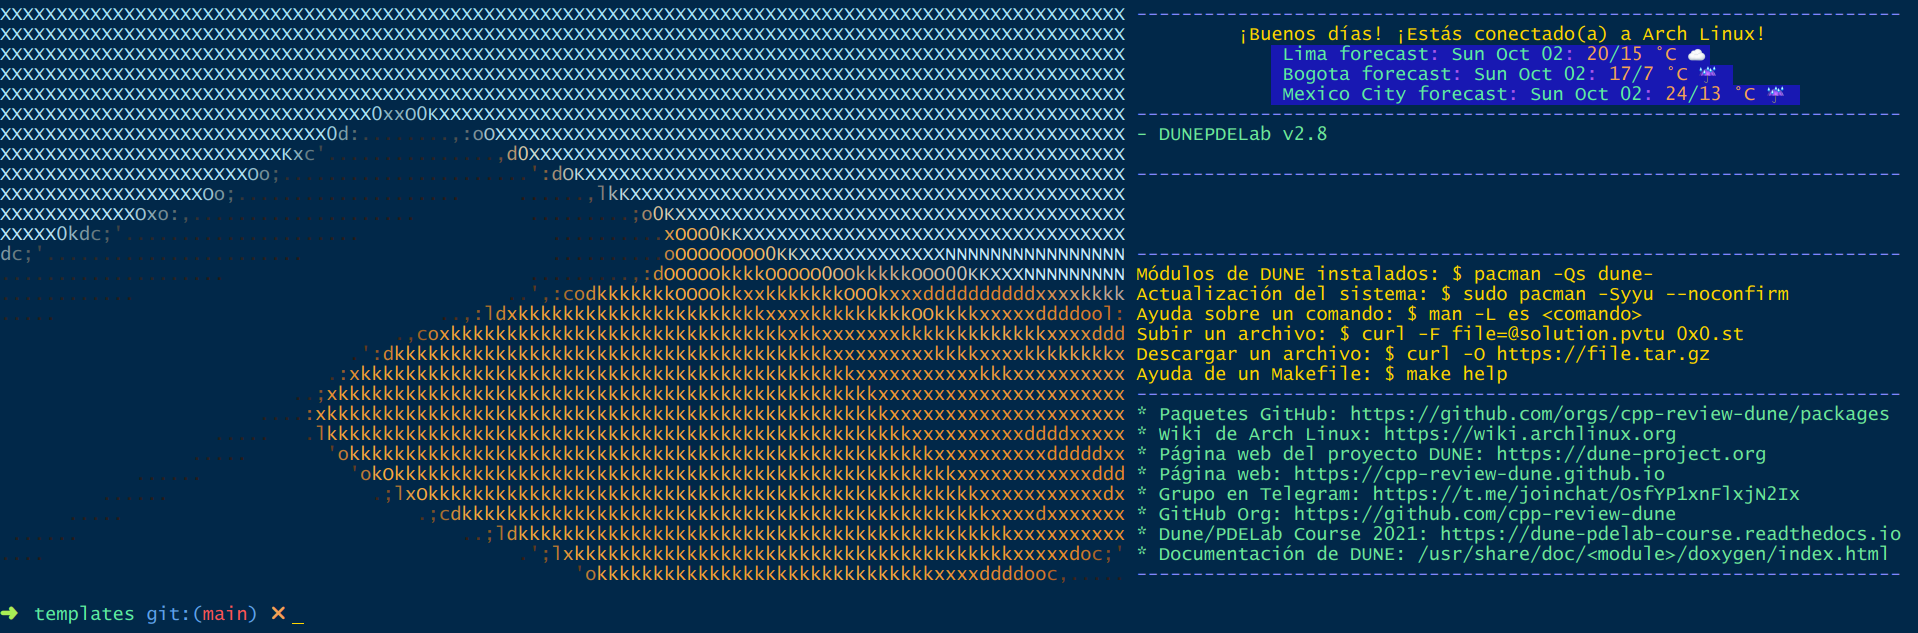
\includegraphics[width=\linewidth]{splash}
		\captionof{figure}{
			C++ Review DUNE says welcome and show useful links to get starting the code inside Gitpod.
			% In diesem Fall sind der Stil {BFH} und BFH-colored identisch
		}

		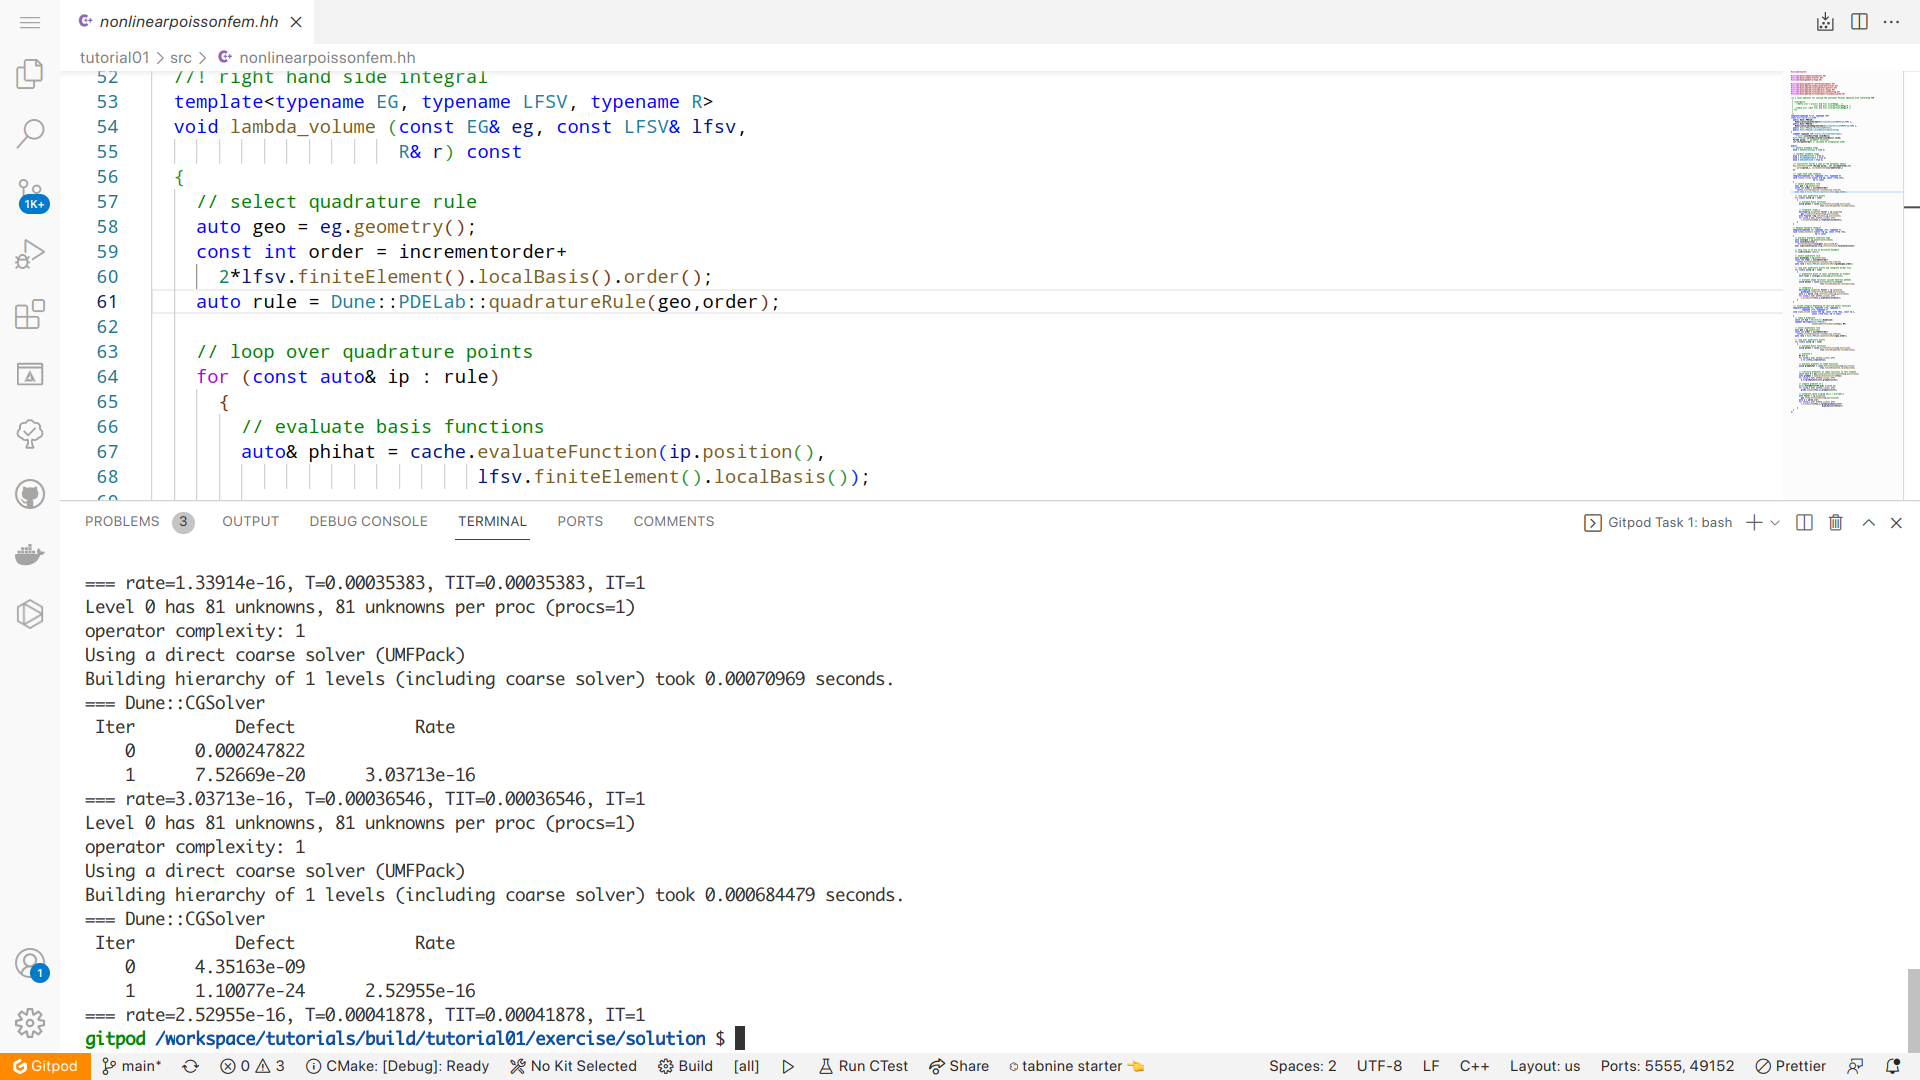
\includegraphics[width=\linewidth]{gitpod-working}
		\captionof{figure}{
			In diesem Fall sind der Stil {BFH} und BFH-colored identisch
		}
	\end{posterboxenv}

	% Eine Box im Stil BFH-framed
	\begin{posterboxenv}[title=A BFH-framed style box, BFH-framed]{name=framed, column=3, row=2, span=2}
		% Die Boxen können in verschiedenen Varianten gestaltet werden. Die Voreinstellung entspricht den offiziellen Vorgaben, jedoch kann es aus unterschiedlichen Gründen notwendig sein, eine klarere Abgrenzung zu setzen (lobale Klassenoption \code{boxstyle=framed} oder lokaler Stil \code{BFH-framed}).
		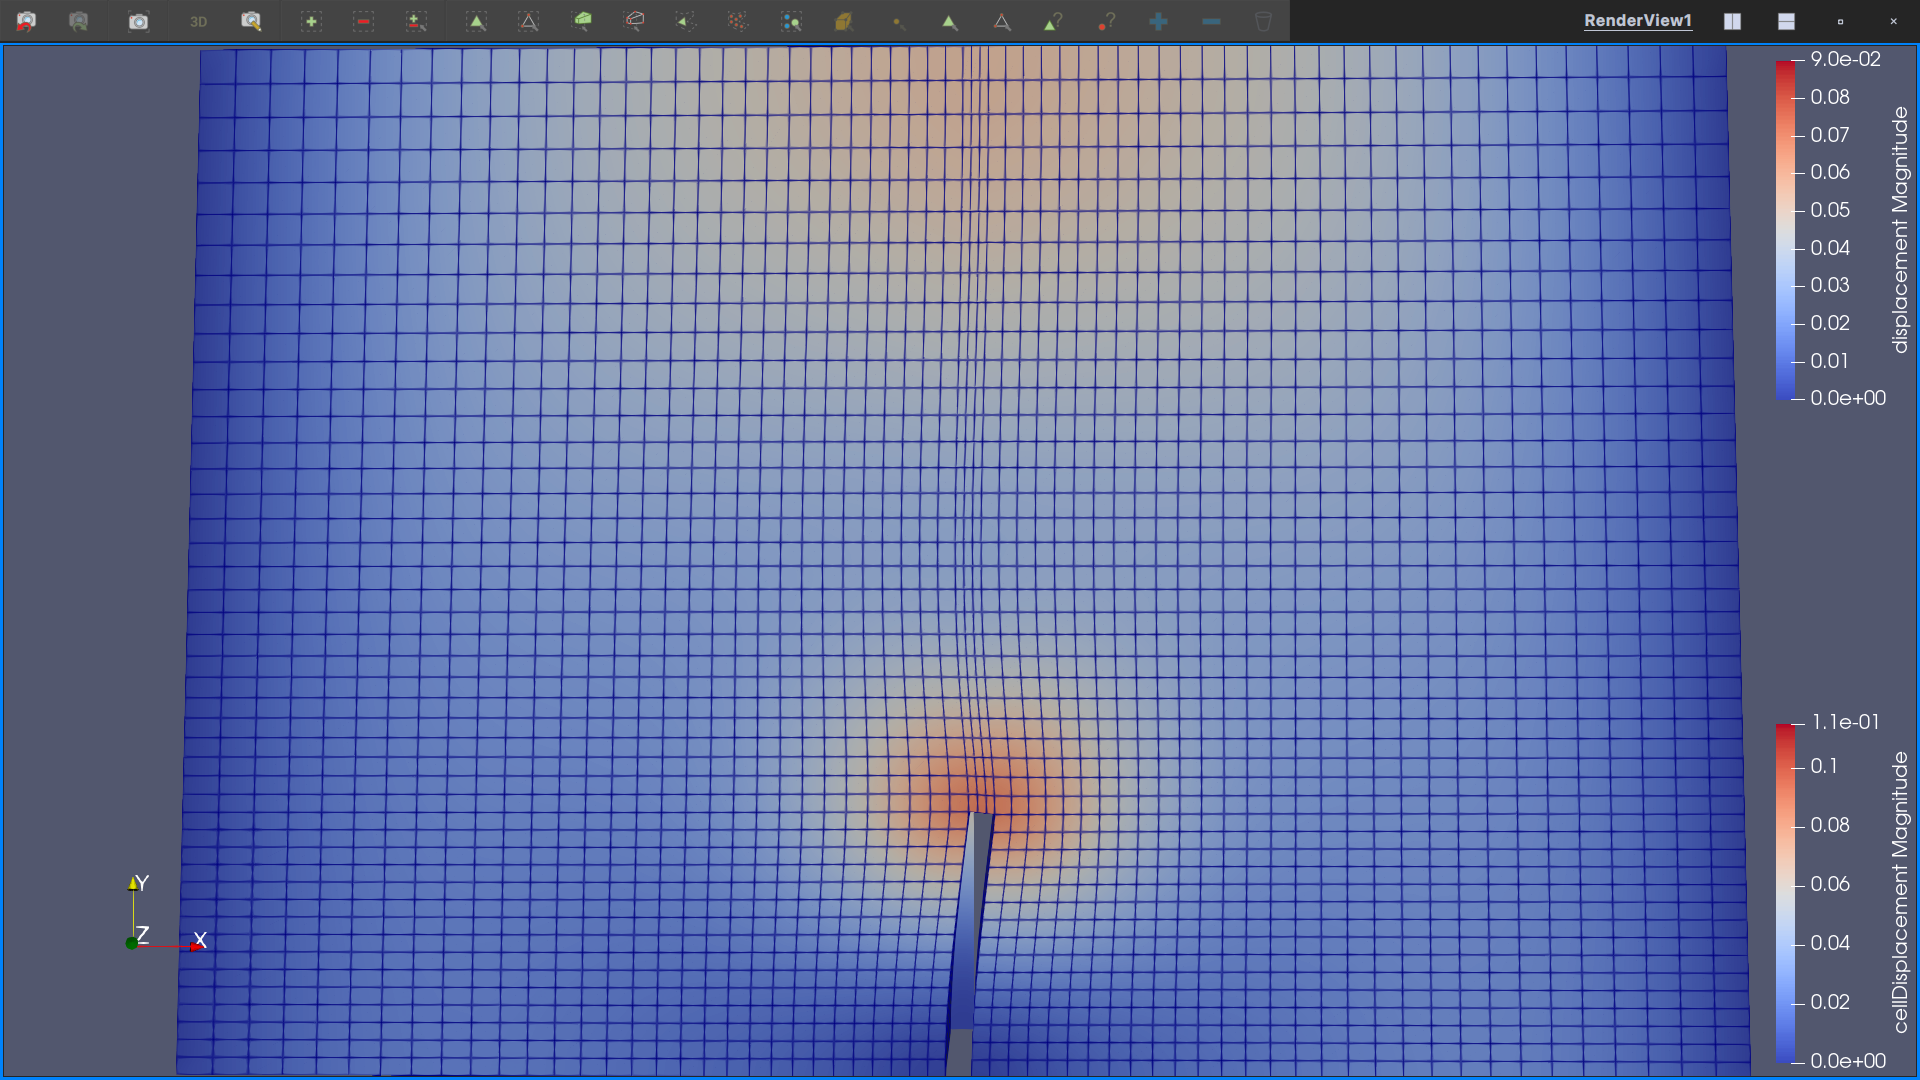
\includegraphics[width=\linewidth]{sequence1}
		\captionof{figure}{
			Example of a fluid-structure interaction, e.g. fluid flowing through a channel in 2D.
		}
		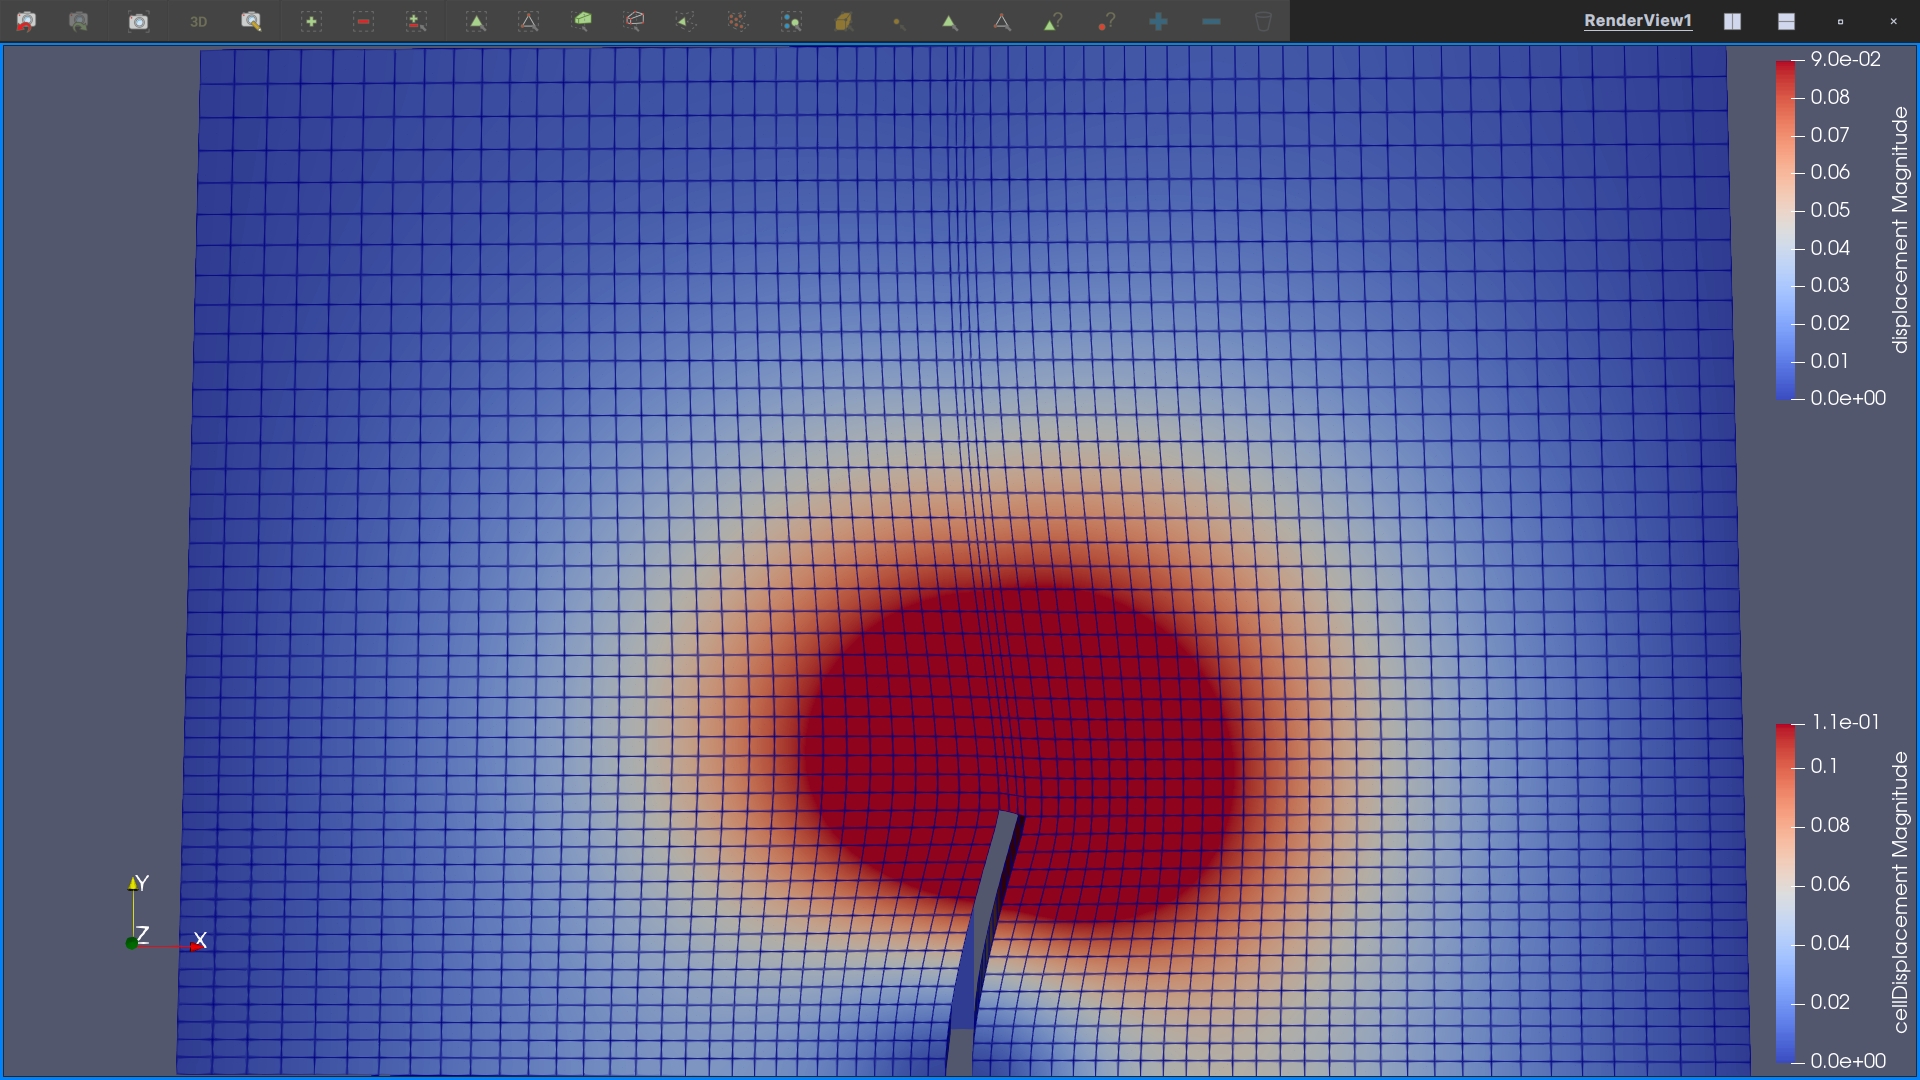
\includegraphics[width=\linewidth]{sequence2}
		\captionof{figure}{
			Example of a fluid-structure interaction, e.g. fluid flowing through a channel in 2D.
		}
	\end{posterboxenv}

	% Fusszeile
	\begin{posterboxenv}[title=Tutorials]{name=footer,below=title, span=2, rowspan=2 }
		% Die Fusszeile ist grundsätzlich aktiviert, kann jedoch mit Hilfe der Klassenoption \code{footer=false} ausgeschaltet werden. In diesem Fall werden jedoch mit \macro{thanks} übergebene zusätzliche Titeldaten nicht angezeigt.

		% Für die Übergabe weiterer Daten stehen die Makros \macro{footer}, \macro{footergraphics} und \macro{footerqrcode} zur Verfügung.

		% \macro{footergraphics} ist für die Übergabe von Logos gedacht und \macro{footerqrcode} übernimmt einen URL die anschliessend in der rechten unteren Ecke als QRCode platziert wird.

		% Die Fusszeile selbst erhält die Daten aus \macro{thanks}, kann jedoch ergänzt werden. Sie hat die Breite des Satzspiegels abzüglich der Logos/QRcode.

		% Der Abstand zwischen Logo und den Inhalten des Fußes, sowie zu den Logos und dem QRcode im Fuß wird über die Länge \macro{footerhsep} gesteuert. Änderung ist über \macro{setlength} möglich.
		\begin{itemize}
			\item \url{https://gitlab.dune-project.org/pdelab/dune-pdelab-tutorials}
			\item \url{https://precice.org/tutorials.html}
			\item \url{https://dune-project.org/sphinx/content/sphinx/dune-fem}
			\item \url{https://amdis.readthedocs.io/en/latest/tutorials/tutorials}
			\item \url{https://www.openfoam.com/documentation/tutorial-guide}
			\item \url{https://github.com/cpp-review-dune/dune-book}
			\item \url{https://git.iws.uni-stuttgart.de/dumux-repositories/dumux-course}
			\item \url{https://github.com/jorgensd/dolfinx-tutorial}
			\item \url{https://parcomp-git.iwr.uni-heidelberg.de/Teaching/hdnum}
			\item \url{https://github.com/cpp-review-dune/cmath-example}
			\item \url{https://github.com/cpp-review-dune/hdnum-examples}
			\item \url{https://github.com/cpp-review-dune/dune-basics}
			\item \url{https://github.com/cpp-review-dune/notebook}
		\end{itemize}

		\url{https://github.com/orgs/cpp-review-dune/packages}
	\end{posterboxenv}

	% Platzierung der Boxen
	\begin{posterboxenv}[title=C++ Review Dune meets Arch4edu]{name=positioning, below=footer, span=2}
		Bei der \pck{poster}-Bibliothek des \pck{tcolorbox} Paketes, werden die Boxen manuell positioniert.

		% Dies benötigt zwar einen zusätzlichen Arbeitsschritt, erlaubt jedoch einer feinere Ausrichtung der Boxen, auch relativ zueinander.

		% Diese Mechanismen ermöglichen auch, Querverweise einfacher zu positionieren. Hierfür ist ein Blick in die \pck{tcolorbox}-Dokumentation hilfreich.
	\end{posterboxenv}

	%% Eine Box im Stil BFH-colored
	\begin{posterboxenv}[title=A BFH-colored style box, BFH-colored]{name=colored, column=3, row=3, span=2}
		Boxentyp zwischen dem Stil \code{framed} und dem Stil \code{official}.

		Einstellung dieser Option ist sowohl über die Nutzung der globalen Klassenoption \code{style=colored} als auch durch die Verwendung des lokalen Stils\code{BFH-colored} möglich.

	\end{posterboxenv}
	%
	% Box ohne Titel mit Abbildung
	% \begin{posterboxenv}[BFH-colored]{name=colored-notitle,column=3,row=4, rowspan=2}
	% 	
\includegraphics[width=\linewidth]{cpp_logo}
	% 	\captionof{figure}{
	% 		Ein Beispielbild, in einer Box ohne Titel (\code{framed-notitle}).
	% 		% In diesem Fall sind der Stil {BFH} und BFH-colored identisch
	% 	}
	% \end{posterboxenv}

	% Box ohne Titel
	% \begin{posterboxenv}[BFH-framed]{name=notitle, column=4, below=colored}
	% 	Ein Beispiel für den Stil \code{framed} ohne einen eigenen Titel.
	% \end{posterboxenv}

	% Box mit Verweis
	% \begin{posterboxenv}[title=Box with reference,BFH-framed]{name=verweis,column=4, above=row6}
	% 	Beispielbox mit Pfeil, um zwei Boxen miteinander zu verknüpfen oder Leseabzweigungen zu generieren.
	% \end{posterboxenv}

	% Zwischen den Boxen kann direkt TikZ-Code eingegeben werden. Das Namensschema der Boxen als Koordinaten lautet
	% TCBPOSTER@<boxname>.ankerpunkt
	% Für genauere Erläuterungen zur Syntax, bietet die tikz-Anleitung genauere Angaben, weitere benannte Koordinaten finden sich in der tcolorbox-Dokumentation
	% \draw[BFH-Orange,line width=4pt,->] ([yshift=-1cm]TCBPOSTER@verweis.east) -|  ([xshift=1cm]TCBPOSTER@colored.east) -- (TCBPOSTER@colored.east);

	% Relative Positionierung
	% \begin{posterboxenv}[title=Relative Positioning,BFH-framed]{name=relative, column=4, between=notitle and verweis}
	% 	Diese Box wird zwischen den beiden Boxen \code{notitle} und \code{verweis} platziert.
	% \end{posterboxenv}

	% Papierformat
	\begin{posterboxenv}{name=paper,column=3,span=2,below=row5}
		\nocite{*} % Insert publications even if they are not cited in the poster
		\bibliography{\jobname}
		% Die Klasse \cls{BFHsciposter} unterstützt die Papierformate A0, A1, A2 und A3. Der Wert wird über die Klassenoption \code{paper} ausgewählt:
		% \begin{verbatim}
		% paper=a0
		% \end{verbatim}
		% Die Voreinstellung entspricht \code{a1}.
		% Die Änderung des Papierformates ist keine Skalierung, da Schriftgrössen nicht direkt skalieren.

		% Um eine Skalierung eines grösseren auf ein kleineres Design zu erreichen, empfiehlt es sich, das Ausgangsformat beim Druck zu skalieren (Drucken in eine Datei mit Skalierung) oder ggf. die PDF-Datei mit Paketen wie \pck{pdfpages} umzurechnen.
	\end{posterboxenv}

\end{tcbposter}

\end{document}